\documentclass[11pt,a4paper]{globis-book}

\usepackage{graphicx}
\usepackage{subfig}
\usepackage[helvetica]{quotchap}
\usepackage{times}
\usepackage{ethfont}
\usepackage[british]{babel}
\usepackage{longtable}
\usepackage{fancyhdr}
\usepackage{shadethm}
\usepackage{makeidx}
\usepackage[a4paper,portrait,twoside,inner=3.25cm,outer=3.5cm,top=3.5cm,bottom=4.0cm]{geometry}
\usepackage{hyperref}
\usepackage{globis}

\renewcommand{\sectfont}{\sffamily\bfseries\Huge}
\setlength{\shadedtextwidth}{\textwidth}
\setlength{\shadeleftshift}{3mm}
\setlength{\shaderightshift}{3mm}
\addtolength{\shadedtextwidth}{-\shadeleftshift}
\addtolength{\shadedtextwidth}{-\shaderightshift}
\setlength{\parindent}{0pt}
\setlength{\parskip}{5pt}

\sloppy

\pagestyle{fancy}
\fancyhf{}
\fancyhead[LE,RO]{\sffamily\bfseries\small\thepage}
\fancyhead[LO]{\sffamily\bfseries\small\leftmark}
    \fancyhead[RE]{\sffamily\bfseries\small\rightmark}
\renewcommand{\headrulewidth}{0.1pt}
\renewcommand{\footrulewidth}{0pt}

\fancypagestyle{plain}{
    \fancyhf{}
    \fancyfoot[C]{\sffamily\bfseries\small\thepage}
    \renewcommand{\headrulewidth}{0pt}
    \renewcommand{\footrulewidth}{0pt}
}

% Please adapt the following fields if necessary!
\hypersetup{
    pdftitle = Distributed Ph Tree, 
    pdfauthor = Bogdan Vancea,
    pdfsubject = Master Thesis,
    hidelinks,
    plainpages = false,
    bookmarksnumbered = true
} 

\raggedbottom

% Please adapt the following fields if necessary!
\title{Cluster-Computing and Parallelisation for the
    Multi-Dimensional PH-Index}
\category{Master Thesis} 
\author{Bogdan Aurel Vancea}
\email{$<$bvancea@student.ethz.ch$>$}
\professor{Prof. Dr. Moira C. Norrie}
\assistant{Tilmann Zaeschke \\Christoph Zimmerli}
\group{Global Information Systems Group}
\institute{Institute of Information Systems}
\department{Department of Computer Science}
\school{ETH Zurich}
\version{}
\date{\today}
\copyrightyear{2014}

\makeindex

\begin{document}

\frontmatter
\maketitlepage
\cleardoublepage
\pdfbookmark{Contents}{toc}

\chapter*{Abstract}

Here comes the abstract.

\tableofcontents

\mainmatter

% Here comes the content

\chapter{Introduction}
\label{ch:intro}
This chapter briefly describes the context and the motivation of the thesis and presents the objectives that are to be achieved. Finally, section \ref{sec:intro-outline} provides an overview of this thesis.

\section{Motivation}
\label{sec:intro-motivation}
Multi-dimensional data is widely used today, especially in domains like database management systems, geographic information systems, computer vision and computational geometry. When all of the dimensions of the data hold numerical values, this data can be viewed as a collection of points in higher dimensional spaces. Due to this nature, multi-dimensional numerical data provides the possibly of posing more complex queries based on the distance between these points in space. For example, in the context of a geo-information system, one could query for all of the points that fall inside a specific hyper-rectangle or attempt to find the nearest neighbours of an arbitrary query point.

Several point-based multi-dimensional indexing solution have been developed in the latest years, the most prominent being kD-trees~\cite{Bentley1975} and quadtrees~\cite{FinkelB74}. This type of data structures store the multi-dimensional data such that more complex operations, like range and nearest neighbour queries are executed efficiently. The PhTree~\cite{Zaschke2014} is a new multi-dimensional data structure based on the quadtree. In addition to providing support for complex queries, the PhTree is also space-efficient, as its space requirements are sometimes even lower than those of multi-dimensional arrays. 

As technology advances and the world becomes more connected, multi-dimensional data becomes easier to acquire and store. Because of this, it is necessary that multi-dimensional data structure need to store and manage more data than would fit a single machine. However, traditional multi-dimensional indexes like the kD-tree and quad-tree do not cover this use case as they are designed to run on a single machine.

Additionally, in the last few years the processor speed has reached the power wall and processor designers cannot increase the CPU frequency by increasing the number of transistors. Recent advances in processor design have been made by adding more cores on CPU's rather than increasing the processing frequency. Therefore, it is important that contemporary data structures be adapted to multi-core architectures by allowing them to support concurrent accesses. As with the case of the increase storage requirements, traditional multi-dimensional data structures do not support concurrent write operations.

This thesis attempts to provide a solution to these two issues by extending the PhTree multi-dimensional index to run on distributed cluster of machines. Furthermore, the PhTree is also updated to support concurrent access.

\section{Objectives}
\label{sec:intro-objectives}
The previous section has highlighted two challenges currently faced by indexing systems: \textit{high storage requirements} and \textit{support for concurrent access.}. This work proposes the distributed PhTree, a version of the PhTree that can be run on a cluster of machines, making it able to handle data sets that cannot fit in the main memory of a single machine. Moreover, the distributed PhTree should be able to handle concurrent requests. This applies both to requests sent to different machines that are part of the cluster and concurrent requests sent by different clients to the same machine. 

Specifically, the distributed PhTree has to fulfill the following requirements:
\begin{description}
    \item[Cluster capability] The system should run across a network of machines, making use of the memory and processing resources on each machine. Furthermore, the system should attempt to balance the number of multi-dimensional entries that each machine is responsible of.
    \item[Cluster concurrency] The system should be able to support concurrent requests to different nodes of the cluster. Each node should be able to process queries related to the entries that it stores locally.
    \item[Node concurrency] Each node should support multi-threaded read and write access to the entries that it stores.
\end{description} 

As the thesis touches on two main subjects, distribution and concurrency, the main challenges encountered are twofold. From the distribution perspective, the challenges are the identification of suitable entry distribution and balancing strategies, devising efficient algorithms for executing queries across multiple cluster nodes, and the efficient management of a very large number of cluster nodes. For the concurrency perspective, the challenges are the identification of a suitable concurrent access strategy that can maximize the number of concurrent write operations.

\section{Thesis outline}
\label{sec:intro-outline}

This chapter gave an overview of the challenges currently faced by multi-dimensional indexing structures and briefly explained how this work seeks to address them. Additionally, this chapter also presented the main objectives of this thesis. The rest of the thesis is structured as follows:

\textbf{Chapter \ref{ch:background}} provides additional information about the PhTree, its characteristics and supported operations. The second part of this chapter describes relevant previous work done in the areas of distributed multi-dimensional indexes and concurrent data structures.

The design of the distributed PhTree from the point of view of a distributed system is presented in \textbf{Chapter \ref{ch:distindex}}. This chapter presents the chosen data distribution strategy, and also touches on the possible alternatives and the consequences of this choice. Additionally, this chapter provides an overview of how the queries spanning multiple nodes are executed by the system.

The addition of the multi-threaded read and write support for the PhTree is discussed in \textbf{Chapter \ref{ch:concurrency}}. Several concurrent access strategies are discussed, together with their advantages, disadvantages and consistency guarantees.

\textbf{Chapter \ref{ch:implementation}} describes the implementation-specific decisions that were taken during the development process. This chapter also presents the technologies that were used and justifies the technological choices.

The distributed PhTree is evaluated in \textbf{Chapter \ref{ch:evaluation}}. The performance characteristics of the implemented distributed systems as well as those of the implemented concurrency strategy are discussed.

\textbf{Chapter \ref{ch:conclusions}} concludes the thesis by presenting the contribution of this work in the context of distributed multi-dimensional indexing systems. This second part of this chapter discusses possible future contributions.

\chapter{Background}
\label{ch:background}
The first part of this chapter analyses the single-threaded PhTree, a multi-dimensional data structure and the starting point of this work. It provides an overview of its specific characteristics and describes the supported operations.

The second part of this chapter presents the relevant related work in the area of distributed multi-dimensional index and concurrent data structures. 

\section{The PhTree}
\label{sec:background-phtree}

The PhTree~\cite{Zaschke2014} is a novel multi-dimensional indexing structure that focuses on fast retrieval and highly efficient storage. It combines concepts from PATRICIA-tries, quadtrees and hypercubes to encode the multi-dimensional data using bit prefix sharing. Because of this, the storage requirements can sometimes be lower than those of the storage requirements of an array of objects.

An example PhTree storing 2-dimensional 4 bit points is shown in \ref{fig:PhTree-example}. The tree illustrated in this figure stores the points: (0, 4), (3, 4) and (3, 6). However, each point is stored as the \textit{bit interleaving} of its values in all dimensions. Therefore, the bit interleaving of point (3, 6), represented in binary as (0011, 1010) is 01001110. By storing the points under the \textit{bit interleaving} form, the PhTree maps the multi-dimensional points into a 1-dimensional space. The 1-dimensional values will be referred to as \textit{Z-values} as they form the \textit{Z-order space filling curve}. 

\begin{figure}[h]
    \centering 
    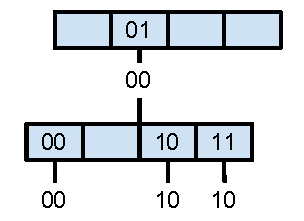
\includegraphics{images/PhTree-example}
    \caption{2 dimensional 4bit PhTree containing the points: (0000, 1000), (0011, 1000), (0011, 1010).}
    \label{fig:PhTree-example}
\end{figure}

The PhTree has the following important properties:
\begin{itemize}
    \item \textbf{Z-Ordering}. The multi-dimensional entries are order according to the Z-order space filling curve. As a consequence, points which are close in the original multi-dimensional space will also be relatively close in the Z-Ordering.
    \item \textbf{Constant height}. The height of the PH-tree is equal the number of bits needed to store each value of the multi-dimensional space. Therefore, when the values in each dimension are represented in 64 bits, as long or doubles, the maximum height of the PhTree is 64. This property is important as \textit{the maximum height of the PhTree is independent of the number of points it stores}.
    \item \textbf{Balancing is not needed}. The PhTree does not perform balancing operation after write operation have occurred. While this fact could lead to un-balanced trees, it is usually not a problem in practice, as the height of tree is limited by a constant factor.
\end{itemize}

The PhTree is similar to a HashMap, as it stores entries consisting of key-value pairs. In this case however, the key is a multi-dimensional data point, while the value can be an arbitrary object. The following operations are supported:
\begin{itemize}
    \item \textbf{Point queries} operate on single multi-dimensional points. The possible queries are \textit{get()}, \textit{put()}, \textit{delete()} and \textit{updateKey()}. The \textit{get()} query retrieves the value associated with a multi-dimensional key, and the \textit{delete()} operation removes the value associated with a multi-dimensional key. The \textit{put()} operation adds new key-value to the index. Finally, the \textit{updateKey()} operations updates the key associated with an existing key-value entry.
    \item \textbf{Range queries} select all of the data points that fall inside a multi-dimensional hyper-rectangle. This rectangle is defined by a \textit{lower left} and a \textit{upper right} point. 
    \item \textbf{Nearest neighbour queries} select the closest k points in the index to an arbitrary query point. 
\end{itemize}

Currently, the amount of entries the PhTree can store limited by the memory available on the host system, as the PhTree stores all data completely in-memory. A distributed version of the PhTree would be able to store a much larger amount of entries and would be able to make use of existing clusters of computing nodes. Specifically, the distributed version would be well suited for running in cloud environments, where users can easily add more computing nodes to their existing systems to handle higher storage requirements and improve performance. The challenges in creating a distributed version of the PhTree are the implementation of range and nearest neighbour queries, which might need to be dispatched to multiple nodes of the system. The goal is to design a set of algorithms that minimize the number of nodes to which a complex query is sent.

\section{Related work}
\label{sec:background-rw}

The following sections reviews the existing research concerning distributed indexes and concurrent data structures. The goal of this section is to understand to existing approaches that can be used for the design and implementation of the distributed PhTre and to identify which of these approaches are best suited for the use cases targeted by this work.
\subsection{Distributed Indexes}

Distributed Hash Tables (DHT's) are a class of decentralized distributed systems which expose an API similar to that of a hash-table. These P2P systems use a structured overlay network to assign a given key to a node in the system. Requests for a certain key can be sent to any node of the system and will be forwarded to the node responsible for it. DHT's have been designed to work on internet-scale, connecting large numbers of machines across large distances. The main concerns are scalability and availability, while the \textit{get()} and \textit{put()} operations have "best effort" semantics. Chord~\cite{Stoica2001chord}, one of the most popular and most efficient DHT system, manages to guarantee that any request for a certain key will arrive the responsible node in at most \textit{O(logn)} hops, in the context in which each nod contains only \textit{O(logn)} links to other nodes. 

One important issues of distributed hash tables is that they only support "exact match" queries. The Prefix Hash Tree~\cite{Ramabhadran04prefixhash} adds support for range queries to a DHT by using a secondary data structure, to maintain a mapping between nodes and keys. This mapping is a trie containing the prefixes of the bit-strings of the keys, and thus, logically, leaf nodes of this trie correspond to interval regions of keys. All leaf-nods are linked using a linked-list, allowing range queries to traverse the query range starting for the first leaf that matches the range. 

A similar approach is taken by the SkipIndex~\cite{Zhang04skipindex}, a multi-dimensional indexing system that uses a SkipGraph to map geometrical regions to machine nodes. Each system node maintains only a partial view of the region tree and thus range and nearest neighbour queries are performed using selective multicasting.

A different approach for creating a scalable multi-dimensional index is to use a big-data platform. \cite{Liao2010HadoopIndex} propose storing a block-based multi-dimensional index structure like the R-tree directly in HDFS and use query models like MapReduce as building blocks for the implementation of range and nearest neighbour queries.

\subsection{Concurrent data structures}

Concurrent data structures are a highly studied problem in current times. Currently, there are two main ways of implementing a concurrent data structures: lock-based solution and lock-free solutions. Lock-based solutions use locks to synchronize the concurrent access to the either the data structure itself, an approach called \textit{course-grained locking}, or to parts of the data structure, in the approach called \textit{fine grained locking}. Lock-free solutions use either atomic primitives, like \textit{compare-and-swap} or software transactional memory to synchronize modification attempts on the data structure.

In the area of concurrent search trees, lock-based approaches are much more common than lock-free solutions. Fraser ~\cite{Fraser2007concurrent} provides a set of API's that can be used to design arbitrary concurrent data structures. While these API's can be used to for any type of data structures, they are based on software transactional memory or multi-word CAS operations, currently not implemented by contemporary hardware. Brown ~\cite{Brown2014concurrent} presents a general technique for non-blocking trees implemented using multi-word equivalents of the \textit{load-link}(LL), \textit{store-conditional} (SC) and \textit{validate}(VL) atomic primitives.

A naive concurrent implementation of a search tree can be achieved by protecting all access using a single lock. Concurrency can be improved by synchronizing the access at the level of nodes. \textit{Hand-over-hand locking}, something also called \textit{lock-coupling}, is a fine-grained technique that states that a thread can only acquire the lock of a node if it holds the lock of the node's parent node. This technique allows multiple concurrent write operations, but the degree of concurrency is limited due to the fact that all subtrees of a locked node are not accessible, even if the other threads need to perform modifications in a different part of the tree. Another approach is to perform optimistic retries by only locking the nodes that should be modified, check if locked nodes have not been removed from the tree and then perform the update. This idea is used by ~\cite{Bronson2010concurrent} to implement a highly concurrent AVL tree.

However, an issue with all concurrent search trees where modifications are done to a single node is that the execution of queries which have to run on the tree for longer periods of time, like iterators or range queries, overlaps with the execution of other write-operatons. Therefore, longer running queries will view the any updates that are done on the tree. In some cases, it is desirable to run the read queries on a snapshot of the tree that is isolated from other concurrent updates. This can be achieved using a strategy called \textit{Copy-On-Write}, which allows a single writer and an arbitrary number of reads to access the same data structure concurrently. Moreover, each write operations creates a new version of the data structure that is only available to readers which have started after the update which created the new version has finished. 

\chapter{Index distribution}
\label{ch:distindex}

This chapter describes the design of the distributed PhTree from the distributed point of view. It presents the challenges and the possible design choices for extending the PhTree to run in a distributed setting, discusses the system architecture and describes the algorithms used for the distributed querries. Concurrency related issues are not tackled in this chapter as they are addressed in Chapter \ref{ch:concurrency}.

\section{Challenges}
\label{sec:distindex-challenges}

While extending the PhTree to be a distributed index increase its storage capacity, there are a number of challenges to overcome in order to reach a good implementation. These challenges are:
\begin{itemize}
    \item \textbf{Balancing the storage load}. In a cluster of n indentical nodes, nodes which have the same hardware resources available, all nodes should store and equal amount of data. Assuming that the values associated with each key are relatively equal in size, all nodes should store a relatively equal number of key-value entries.
    \item \textbf{Maintaining data locality}. The PhTree needs to provide support to range and nearest neighbour queries, types of queries which generally analyze contiguous portions of the space and return sets of points which are generally close together. If the indexed points manifest locality, points close in space reside on the same node, range and nearest neighbour queries could be sent to only a part of the nodes in the cluster. In the best case, range and nearest neighbour queries could be sent to only a single node. It is therefore preferable that queries are sent to as few nodes as possible, minimizing both the response time and the request load to the nodes in the cluster.
    \item \textbf{Ensuring cluster scalability}. To support very large storage requirements, the system should support a large number of online-indexing nodes. Furthermore, to support scalability, adding and removing nodes to and from the system should be easy and should not require the cluster to be shut down and then re-started. Such atomic cluster re-configuration is challenges because of the data migrations that it entails to achieve a balanced storage load. New nodes added to the system start off as being empty and should received some entries from the currently running active nodes. Moreover, the data received should preserve locality. Nodes that are being removed from the system need to first make that the entries currently stored and moved to different nodes in the system in a manner that preserves locality. 
    \item \textbf{Minimizing node information}. As the PhTree is held in-memory, it is important for the indexing nodes to be efficient in managing their memory, to maximize the entries stored by the tree. Maintaining a connection to node over a network generally requires an open socket on both participating nodes. However, active sockets take up system memory and CPU cycles, making it important to reduce the number of open connections that a node has to other nodes in the system. Therefore, it is important to devise a communication model in which each node has to be aware and communicate with a small number of other nodes in the system, to reduce the resource compution related to cluster membership.
\end{itemize}

Other challenges posed by distributed indexes and distributed systems in general are availabilty and security, however these issues are not tackled by this work.

By taking into account the discussed challenges, an ideal architecture of the system has the following requirements:
\begin{enumerate}
    \item Ensure low response time by minimizing the number of network requests that have to be made.        
    \item Points are assigned to nodes in the cluster in a way that preserves locality.
    \item New nodes can be added and removed without shutting down or stopping the cluster.
    \item Each node maintains open connections to a small number of other nodes in the system.
\end{enumerate}

The following sections of this chapter describe the distribution strategy chosen to properly address the challenges presented in this section, the final architecture of the system and the algorithms for the query execution.

\section{Distribution strategies}
\label{sec:distindex-strategies}

There are two main solutions to the problem of distributing a tree data structure over a cluster of computing nodes: 
\begin{itemize}
    \item \textbf{Assigning tree nodes to machines}. In this approach, there will be only a single PhTree containing all of the entries stored by the cluster, each node of the PhTree being stored on an individual machine. This means that following a pointer from a parent tree node to a child tree node could require the forwarding of the request to a different machine, the one containing the child tree node. As the PhTree depth is limited by a bit width of the data being stored, from the theoretical point of view, the number of such "forwards" is limited by a constant number. Additionally, spreading the tree nodes uniformly across the machines will lead to a balanced storage load. The drawback of this approach is that even though the number of "forwards" during a tree travels is limited by a constant number, the impact on the response time of the system is very high as each "forward" constitutes of a network request. For example, for indexes storing 64 bit multi-dimensional points, a point query would take 64 forwards between the machines in the cluster in the worst case.  
    \item \textbf{Assigning data points to machines}. In this approach, each machine in the system will maintain a in-memory PhTree and data points are assigned to machines according to some mapping. This mapping will be referred to as the \textit{key-mapping}, as it mantains a mapping between the keys of the entries stored and the machines that store them. Queries for arbitrary points will always be dispatched to the machines that hold the poins, according the \textit{key-mapping}. Therefore, if the \textit{key-mapping} is known by the clients of the index, point queries can be resolved by a single "network" request. However, in such an architecture, the manner in which the points are distributed according to the \textit{key-mapping} influences the manner in which the range and nearest neighbour queries are executed. 
\end{itemize}

While both of these alternatives satisfy some of the requirements of an ideal architecture, the drawbacks of the first approach, the assignment of tree nodes to machines, outweigh the advantages it provides. The number of network requests needed by this approach when storing 32 or 64 bit data, typical for most applications, make the use of this approach prohibitive in a setting where queries must have a low-latency.

Therefore, this work will focus on the second distribution approach. The following sections will present possible strategies for distributing the points to PhTree's store on different machines in the cluster.  

\subsection{Hashing}

The first approach considered is using a \textit{hashing} function to assign the multi-dimensional points to machines in the clusters. This process is illustrated in figure \ref{fig:hashing}. The hashing function takes the multi-dimensional point and generates a host id h based on the point values in each dimension. This approach is similar to the approach used to implement in-memory hash tables, where keys are mapped to buckets in the hash table.

The main advantage of this approach is that if the hash function is known to all of the machines in the cluster and to all of the clients, point queries can be executed in O(1) network requests. Moreover, if the hash function is uniform, the multi-dimensional points are spread uniformly across the cluster, leading to a balanced storage load on all of the machines.

However, the use of a hash function for the point distribution presents some drawbacks. First of all, a hash function works well for a fixed number of hosts n. A different cluster configuration, with a different number of machines, requires the use of a different hash function. Moreover, changing the hash function requires a re-hashing of all of the points already stored in the cluster, potentially leading to a situation where all of the stored points need to be moved to a different machine. This situation would case a lot of traffic within the cluster, making it hard for the system to answer queries until the migration process is finished.

\begin{figure}[h]
    \centering 
    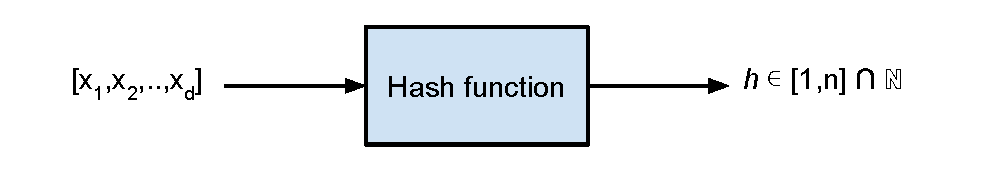
\includegraphics[scale=0.9]{images/hashing}
    \caption{Distributing the points based on a hash function}
    \label{fig:hashing}
\end{figure}

A second issue with use of hash functions is the observation that hash functions which are perceived to be good in this situation spread the multi-dimensional points uniformly across the machines in the cluster. In such a situation, is is quite likely that the hash function does not preserve point locality, and such, complex queries like range queries and nearest neighbour queries will need to be dispatched to all of the computing nodes in the cluster. 

\subsection{Spatial splitting}

Another approach that can be used for the point distribution problem is to split the partition the original space into a set of contiguous regions and assign each region to a hosts in the system. The most intuitive way to perform this split is to split the multi-dimensional space equally to obtain one region per index host. Figure \ref{fig:geometric-2hosts} shows a potential splitting of a 2D space for 2 hosts, while Figure \ref{fig:geometric-4hosts} presents a possible split of the same 2D space for 4 hosts. 

\begin{figure}
\centering
\parbox{5cm}{
    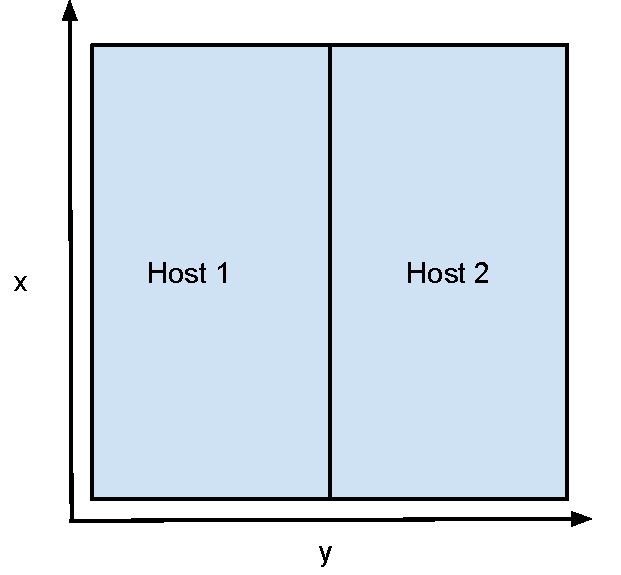
\includegraphics[width=5cm]{images/geometric-2hosts}
    \caption{Equal geometric space splitting for 2 hosts and 2 dimensions}
    \label{fig:geometric-2hosts}}
\qquad
\begin{minipage}{5cm}
    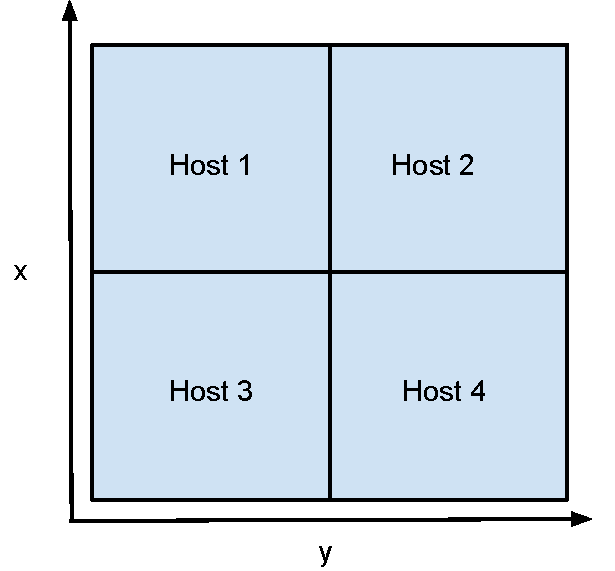
\includegraphics[width=5cm]{images/geometric-4hosts}
    \caption{Equal geometric space splitting for 4 hosts and 2 dimensions}
    \label{fig:geometric-4hosts}
\end{minipage}
\end{figure}

The spatial splitting approach is not only intuitive, but it also preserve locality, as generally, points which are close together are part of the same regions and are therefore stored on the same machine. Additionally, range queries can be resolved by dispatching the range query to all of the hosts whose assigned regions intersect with the range received as input. In the best cases, range queries can be dispatched to a single host. It is generally preferable to split the space into hyper-rectangles, as these regions can be stored using only two data points, the top left and bottom right corners, independently of the number of dimensions of the original space. 

While the spatial splitting works well in some situations, sometimes it is unclear how to properly split the space between the machines. For example, the 2D space is easy to split into 2 or 4 equal regions, but it is more difficult to split for 3 or 5 hosts. It is always possible to split the space into n equal sized "strips", however this approach diminishes the locality of the data for large values of n. Representing regions as arbitrary polygons instead of hyper-rectangles addresses the problem to a degree, but storing these polygons and computing intersection between them is more difficult than performing the same task using hyper-rectangles. 

Difficulties in splitting the space can also arise even when using hyper-rectangle regions of different size. One instance is the case skewed point distributions, presented in figures \ref{fig:geometric-bad-split} and \ref{fig:geometric-bad-split-2}. In the case of the point distributions illustrated in these figures, an equal space split would not split the points equally between the hosts. However, there are many possible rectangle-based splittings of the space, and it is unclear which of these it is better. In some case, the best split could be achieved by splittng the space into more regions than machines and assign each region to a machine.

\begin{figure}
\centering
\parbox{5cm}{
    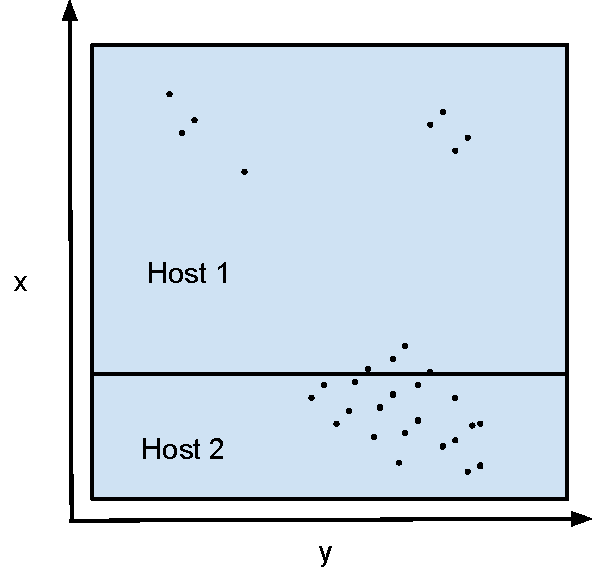
\includegraphics[width=5cm]{images/geometric-bad-split}
    \caption{}
    \label{fig:geometric-bad-split}}
\qquad
\begin{minipage}{5cm}
    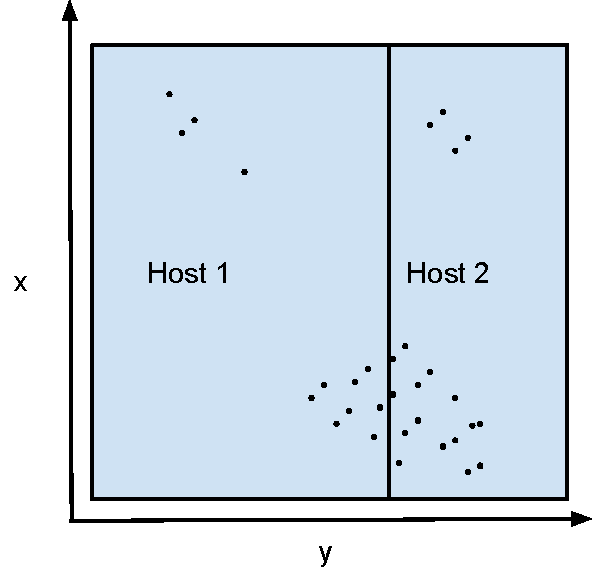
\includegraphics[width=5cm]{images/geometric-bad-split-2}
    \caption{Equal geometric space splitting for 4 hosts and 2 dimensions}
    \label{fig:geometric-bad-split-2}
\end{minipage}
\end{figure}
        
Additionally, in the case of skewed input distributions, the optimal split of the space into regions will change over time, as some regions will end up containing more and more points. In this case, the cluster needs to go through a \textit{re-balancing} phase, when the regions are modified and some points are moved from highly populated regions to less populated neighbouring regions. An important observation is that the number of neighbouring regions for an arbitrary regions is a function of the number of dimensions of the original space. This leads to a large number of regions participating, or at least being considered, in the re-balancing of the points from a single dense region to its neighbours. 

\subsection{Z-Order curve splitting}

As previously mentioned, the in-memory PhTree stores the multi-dimensional points according to the Z-ordering, by mapping the initial space to the 1-dimensional Z-order curve. This curve fills in the initial space in a contiguous and complete manner. Figure \ref{fig:zordering-clear}\footnote{Image adapted from \url{http://www.scholarpedia.org/article/B-tree_and_UB-tree}} shows the Z-order space filling curve filling the 2D space where the values in each dimension are limited by 3 bits.  

\begin{figure}
    \centering
    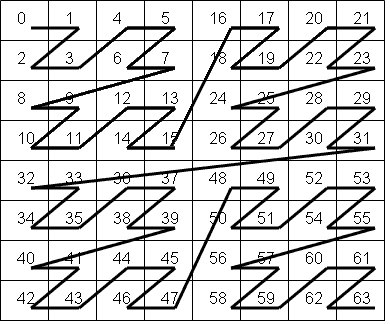
\includegraphics[scale=0.8]{images/zordering-clear}
    \caption{Z-order space filling curve filling the 2 dimensional space.}
    \label{fig:zordering-clear}
\end{figure}

Therefore, instead of splitting the original space into regions, one could attempt to parition the z-order curve into contigous intervals. Figure \ref{fig:zorder-line} shows the 1 dimensional z-order curve corresponding same 3 bit 2-dimensional space, split into 4 intervals of different colours: $[{0, 12}]$ with blue, $[13, 35]$ with yellow, $[36, 47]$ with violet and $[48, 63]$ with green. Figure \ref{fig:zorder-square} shows how the interval splitting is reflected in the original space. Each interval on the z-order curve corresponds to either a hyper-rectangle or a set of hyper-rectangles. Each interval in the z-order curve is reprsented by at most $O(d*w)$ hyper-rectangles, where d is the number of dimensions and k is the number of bits needed to represented the values in each dimension. ~\cite{skopal2006-ubtree} provides an algorithm for generating the hyper-rectangles associated with a z-order curve range.

\begin{figure}
    \centering
\parbox{5cm}{
    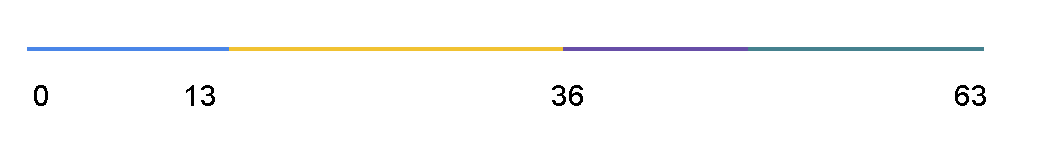
\includegraphics[width=5cm]{images/zorder-line}
    \caption{Example intervals on the 3bit z-order curve}
    \label{fig:zorder-line}}
\qquad
\begin{minipage}{5cm}
    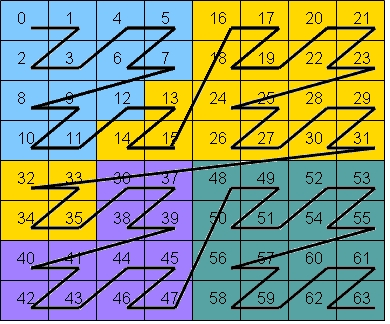
\includegraphics[width=5cm]{images/zorder-square}
    \caption{Example intervals on the 3bit z-order curve filling the 2D space}
    \label{fig:zorder-square}
\end{minipage}
\end{figure}

An advantage of this splitting method is the regions corresponding to the z-order intervals manifest locality, making it well suited for a point distribution method. Moreover, even if in the original space each region has O(d) neighbours, each interval on the z-order curve has a small, constant number of neighbouring intervals (2 for the interior intervals, 1 for the two edge intervals). This makes it easier to handle the cases in which a region is densely populated and should re-balance its points to neighbouring regions. 

Due to the presented advtanges, the z-order curve interval splitting is the method that was chosen as a point distibution strategy for the distributed PhTree. 
\section{Architecture}
\label{sec:distindex-architectures}

The network architecture of the distributed PhTree is presented in Figure \ref{fig:architecture}. The points are distributed to the hosts in the cluster using the z-order curve interval splitting method. The \textit{key-mapping} is stored on the configuration server and is known to all of the nodes and the clients of the system. The configuration server uses a notification-based model and is responsbile for notifying the indexing hosts and clients whenever any changes occur. This model reduces the amount of network traffic within the cluster, as nodes and clients only need to read the \textit{key-mapping} on start-up and do not need to poll the configuration server for changes. 

Clients of the index first connect to the configuration server, retrieve the \textit{key-mapping} and register to receiver notifications if the mapping changes. After receiving the mapping, clients can begin to send queries to the indexing nodes within the cluster. Clients decide which hosts need to the contacted for a query based on the type of the query and the \textit{key-mapping}. This model is efficient as it allows the clients to decide the hosts to be queried based on local data. Futhermore, queries concerning more indexing nodes can be executed by sending network requests in parallel to all of the involved nodes. A potential drawback of this model is that the configuration server could become the bottleneck in a system with many indexing hosts or many connected clients. This issue can be addressed by using replicating the configuration data to a cluster of configuration servers. An alternative solution would be to store only a partial representation of the mapping in each indexing node and allow queries to be "hop" from one node to the other until they reach the destination machines, as in the case of the prevously discussed distributed hash tables. However, the extra latency introduced by repeated "hops" with the cluster makes this approach ill-suited for latency-sensitive applications like a distributed-index.  

\begin{figure}[h]
    \centering 
    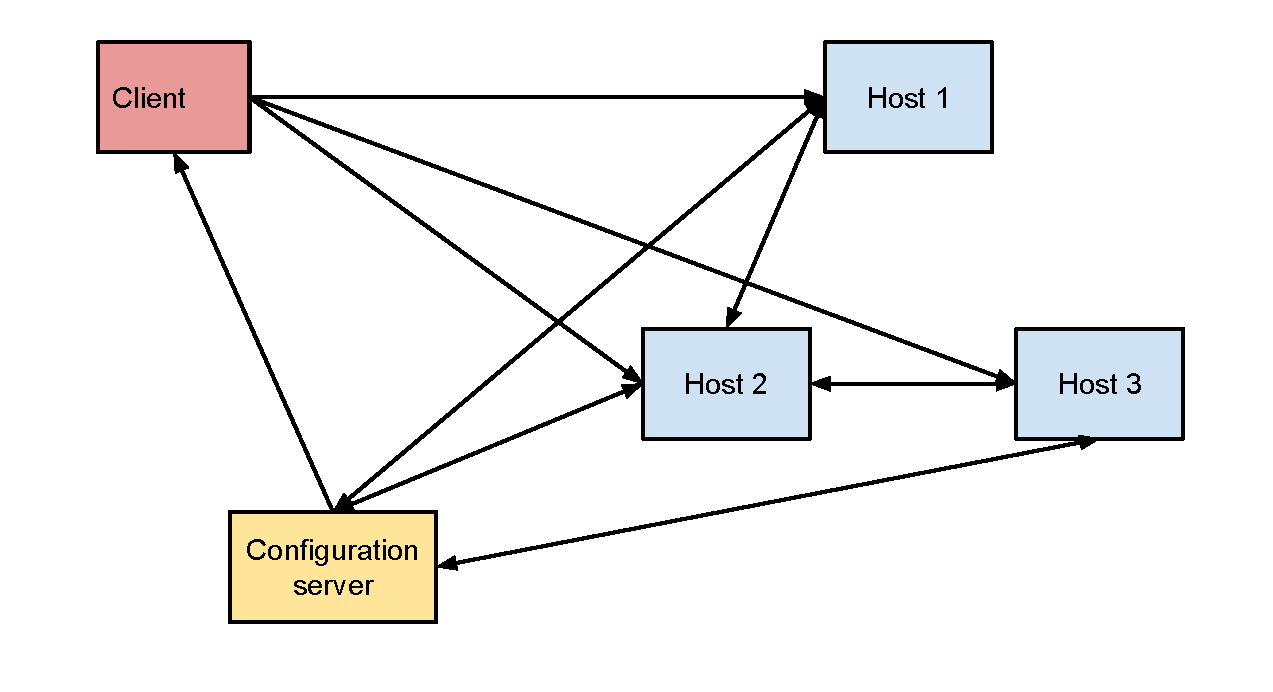
\includegraphics[scale=0.7]{images/architecture}
    \caption{The architecture of the distributed PhTree}
    \label{fig:architecture}
\end{figure}

As the data is split according to z-order curver intervals, each indexing hosts only needs to maintain two connections to other hosts in the cluster (or 1 for the hosts holding the edge intervals). This means that the amount of memory used by the hosts to store cluster membership information remains relatively constant, even if the number of the nodes in the cluster increases. 

\section{Algorithms}
\label{sec:distindex-algorithms}

This section will discuss how the \textit{key-mapping} is created from the Z-order curve intervals and how the queries are executed based on the key-mapping. 
\subsection{Key-mapping design}

The \textit{key-mapping} used by the distributed PhTree assigns the points based on the Z-order curve intervals. To determine the host responsible for a certain multi-dimensional point, one would have to map that point to the Z-order curve and determine the interval that contains it. There are two alternative for designing the \textit{key-mapping} based on the Z-order curve intervals:
\begin{enumerate}
    \item Store the Z-intervals directly as pairs of Z-values and perform 1-dimensional interval matchings to determine the hosts that have to be contact for certain queries. The operation is linear in the number of hosts, for both point and range queries, as the Z-values of the query points need to be compared with the Z-values of the intervals. The correctness of this approach stems from the fact that the region represented by a d-dimensional hyper-rectangle [X, Y] \footnote{Where X is the top-left corner of the hyper-rectangle and Y is the bottom-left corner of the hyper rectangle} is included in the set of d-dimensional regions corresponding to Z-interval $[Z_X,Z_Y]$.
    \item Store the hyper-rectangles from the original space that correspond to each Z-order interval and perform intersections between the query points/rectangles from the original space and the hyper-rectangle of the interval regions. This operation takes $O(n * w * d)$, as each region contains at most $O(w * d)$ hyper-rectangles. 
\end{enumerate}

Even if the first solution is asymptotically faster than the second one for finding the hosts to query, the first approach attempts to query a much larger area in the original space than the second one. Therefore, the first method can potentially generate many more network requests than the first one, especially in a system with a large number of online indexing hosts. Moreover, the intersection operation itself is performed on the client, in-memory, and does not generate a network request. Because of these reasons, the second approach is preferable to the first approach in a system looking to minimize the number of network requests associated to each query, like the distributed PhTree. 

\subsection{Point queries}
Point queries involve operations on a single query point, the insertion or removal of a key-value pair, obtaining the value associated with a key value pair or changing the key associated with a key-value pair. For the point queries, the client only needs to determine which host to send the request to. This is done by determining the intersections between the query point and the hyper-rectangles corresponding to the Z-order intervals. In the case of the \textit{get()}, \textit{put()} and \textit{delete()} operations, the client sends the request to the hosts responsible for the query point and returns the result of the operation. In the case of the \textit{updateKey()} operations, it is possible that a different host is currently responsible for the new key of the value associated with the query point. In that case, the \textit{updateKey()} operation is performed in two steps: first the client removes the old key from the host responsible for it, and the inserts the new key to the proper host.

\subsection{Range queries}

\subsection{Nearest neighbour queries}

\subsection{Entry load balancing}


\chapter{Concurrency}
\label{ch:concurrency}

\textit{Meta - will be removed after editing.}
\textit{Present the concurrency strategies that could be added to the PhTree and explain the consistency model associated with each strategy.}

The PhTree does not currently support concurrent write operations. There are several strategies that could be employed to add concurrent writes.

\section{Challenges}

\section{Concurrency strategies}

\subsection{Copy-on-Write}

\begin{figure}[h]
    \centering 
    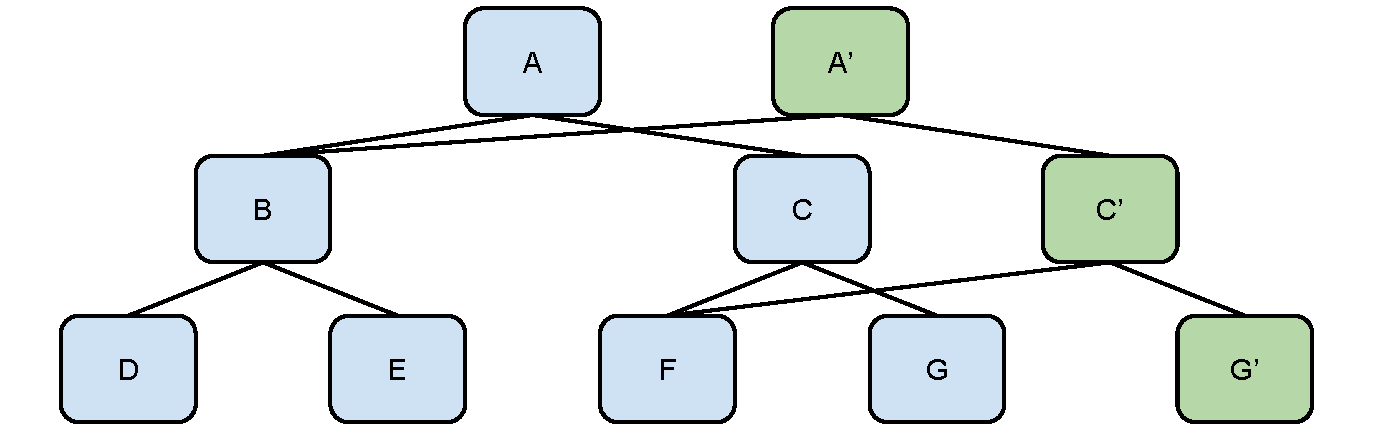
\includegraphics[scale=0.6]{images/Tree-COW}
    \caption{Illustration of Copy-on-Write on a binary tree}
    \label{fig:tree-cow}
\end{figure}

\subsection{Locking}
\begin{figure}
    \subfloat[caption]{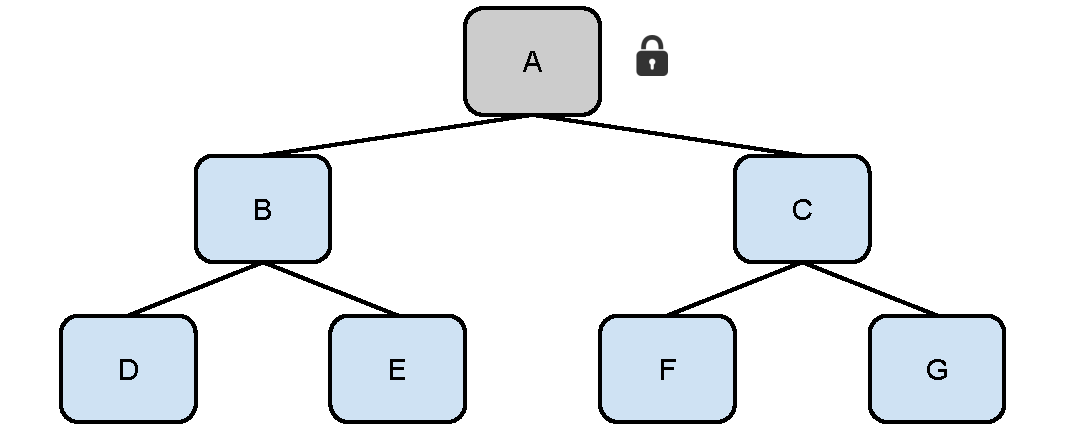
\includegraphics[width = 2in]{images/Tree-HoH-a}}
    \subfloat[caption]{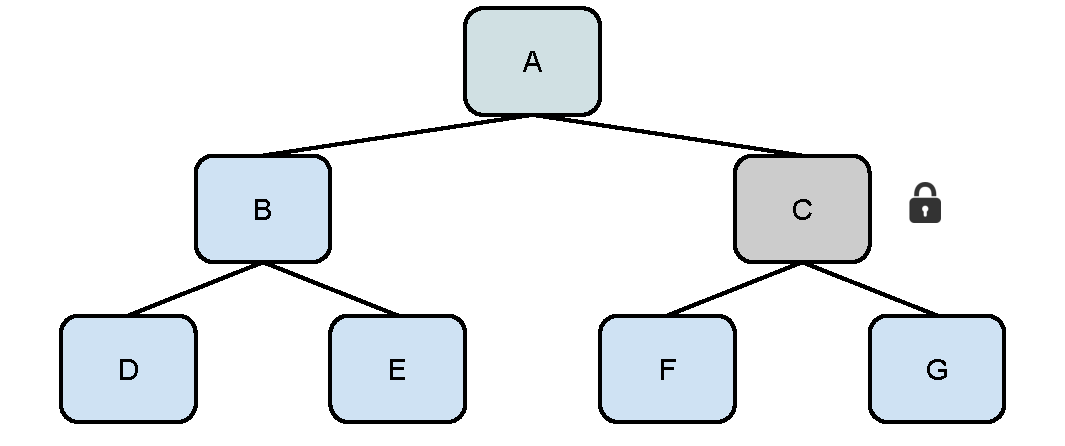
\includegraphics[width = 2in]{images/Tree-HoH-b}}
    \subfloat[caption]{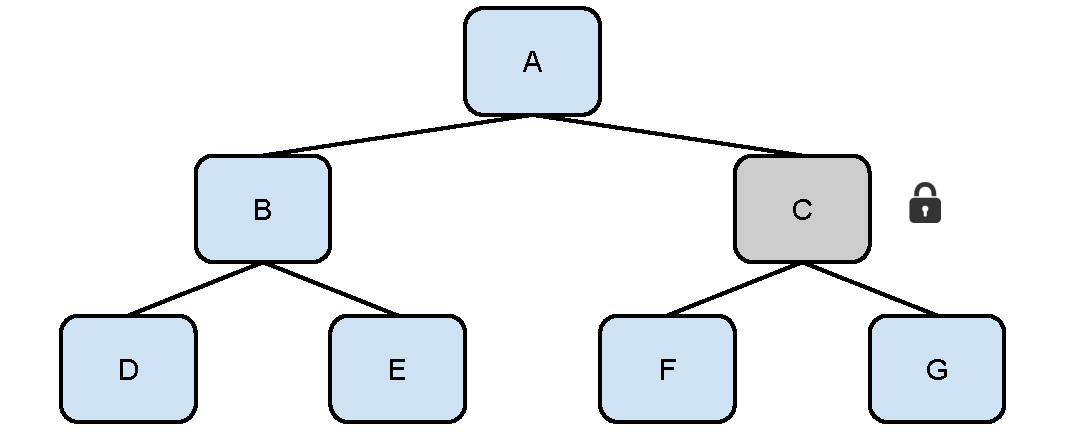
\includegraphics[width = 2in]{images/Tree-HoH-c}}
\caption{}
\end{figure}
\chapter{Implementation}
\label{ch:implementation}

\textit{Meta - will be removed after editing.}
\textit{Present the implementation architecture and the techologies used.}

\section{System description}
\textit{Meta - will be removed after editing.}
\textit{Describe the system, include class/deployment diagrams.}

\begin{figure}[h]
    \centering 
    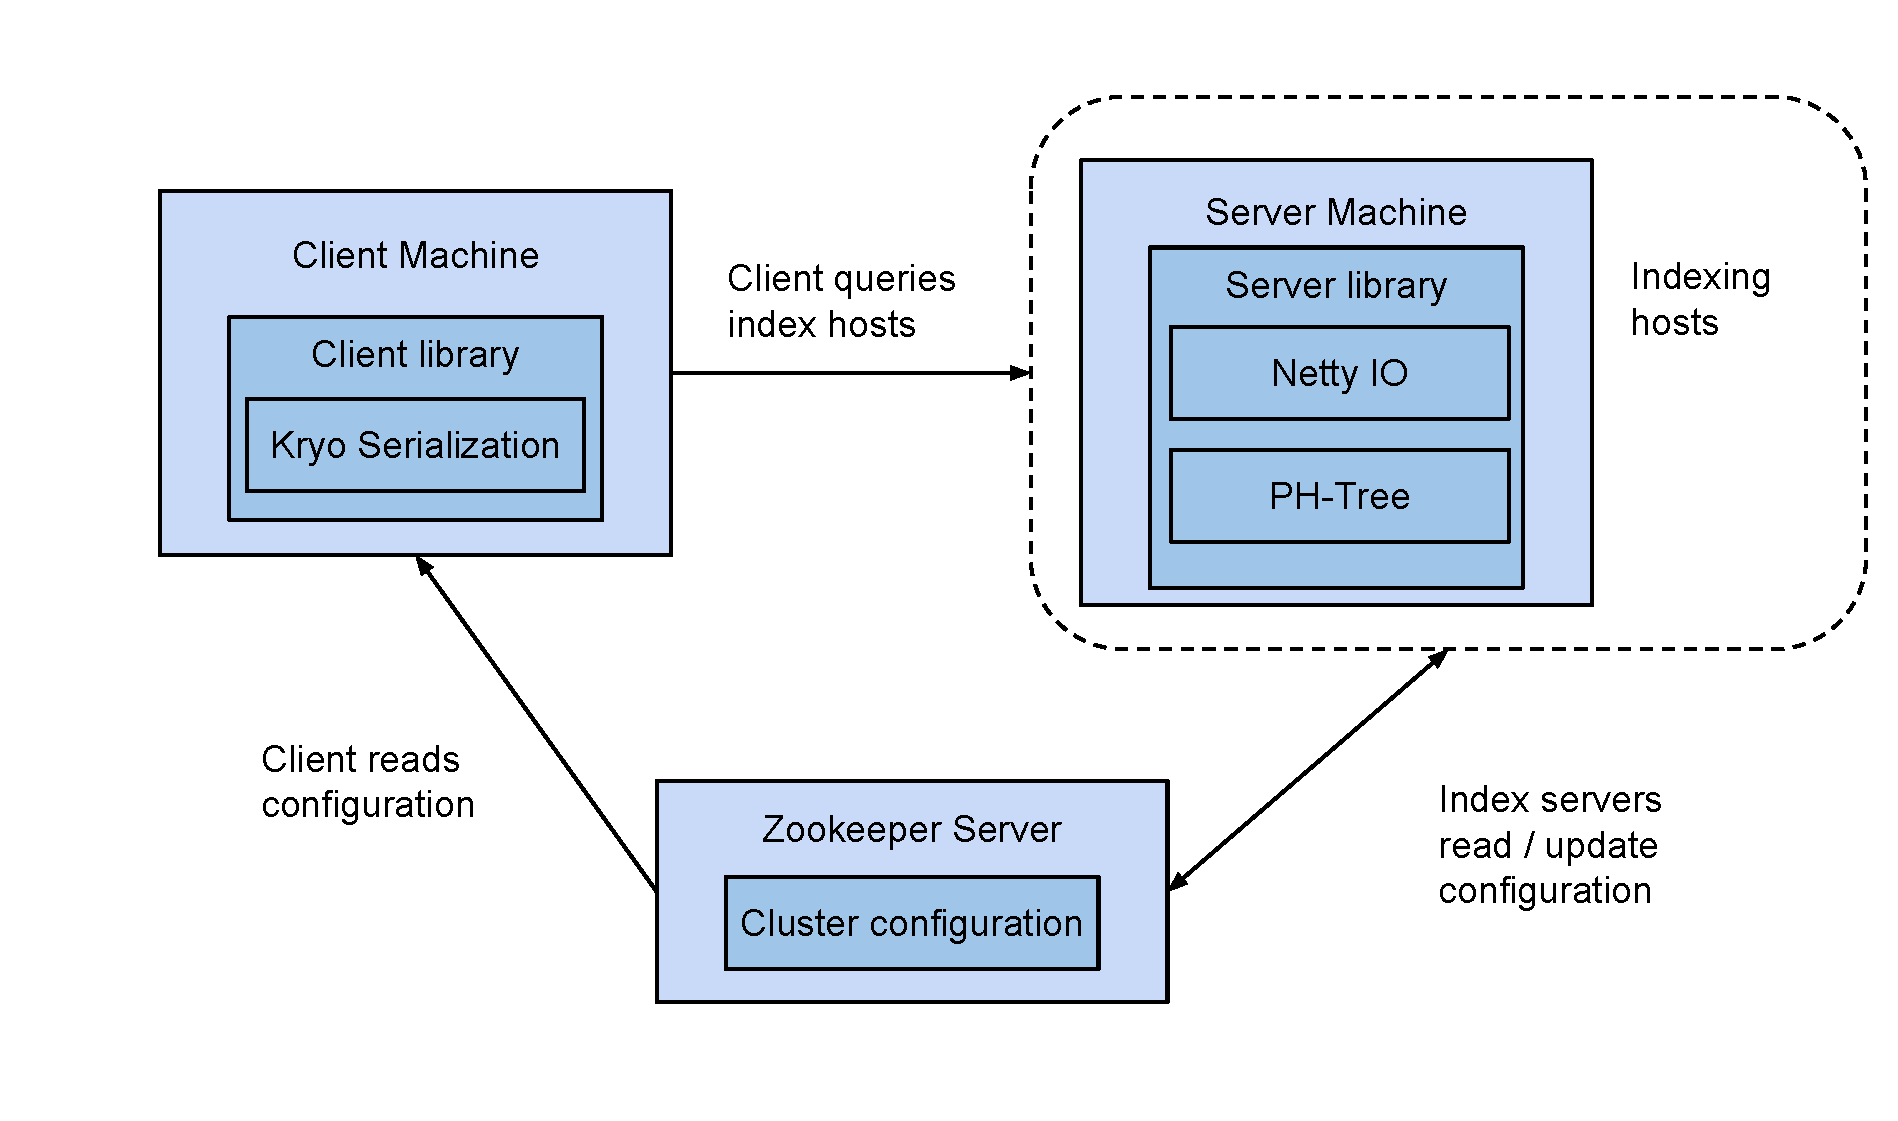
\includegraphics[scale=0.4]{images/implementation-architecture}
    \caption{The implementation architecture of the distributed PhTree}
    \label{fig:implementation-architecture}
\end{figure}
\section{Technologies}
\textit{Meta - will be removed after editing.}
\textit{Describe the technologies used, the reasons for which these technologies were chosen and any alternatives.}

\chapter{Evaluation}
\label{ch:evaluation}

\textit{Meta - will be removed after editing.}
\textit{Explain how the system should be evaluated, present and explain the benchmarks}

\chapter{Conclusions}
\label{ch:conclusions}

\section{Contributions}
\label{sec:conclusions-contribution}
\textit{Meta - will be removed after editing.}
\textit{Conclude the report. This should reiterate the main points of the report and try to mirror the introduction}

\section{Future work}
\label{sec:conclusions-future-work}
\textit{Meta - will be removed after editing.}
\textit{Present the points that were not tackled by the thesis and talk about possible future work.}

\appendix

\listoffigures
\listoftables

\chapter*{Acknowledgements}

\newpage
\thispagestyle{empty}

\bibliographystyle{plain}
\bibliography{bibliography}

\end{document} 
